\documentclass[12pt]{article}
\usepackage{xeCJK}

\usepackage{charter}
\usepackage{fullpage}
\usepackage[colorlinks=false]{hyperref}
\usepackage{ifthen}
\usepackage{comment}
\usepackage[title,titletoc]{appendix}
\usepackage{pagecolor}
\usepackage{amsmath}
\usepackage{amsfonts}
%\usepackage[normalem]{ulem}
\usepackage{siunitx}
\usepackage{amsthm}
\usepackage{paralist}
\usepackage[numbers,sort&compress]{natbib}
\sisetup{per=slash, load=abbr}

\usepackage{pgfplots}
\usetikzlibrary{positioning}
\usetikzlibrary{fit}
\usetikzlibrary{snakes}
\usetikzlibrary{shapes.geometric}
\usetikzlibrary{patterns}
\usetikzlibrary{shapes,arrows,chains}
\usepgfplotslibrary{patchplots,colormaps}
\usetikzlibrary{calc}
\usetikzlibrary{positioning, fit}
\usetikzlibrary{backgrounds}
\usetikzlibrary{intersections}

\newcommand{\whitepaper}[1]{\begin{center}\fbox{\parbox{0.75\textwidth}{{\small
#1}}}\end{center}}

\newcommand{\pcolor}{white!25}

\usepackage{setspace}
\usepackage{algorithm2e}
\bibliographystyle{ieeetr}

\usepackage{geometry}
\geometry{left=3cm,right=3cm,top=1.6cm,bottom=3cm,headheight=0pt,headsep=1.5em}
\usepackage{fancyhdr}
\pagestyle{fancy}

\usepackage{indentfirst}


\setCJKmainfont[BoldFont = STSongti-SC-Bold]{STSongti-SC-Regular}
\setCJKfamilyfont{hei}{SIL-Hei-Med-Jian}		%宋体
\setCJKfamilyfont{song}{SimSun}		%宋体
\setCJKfamilyfont{kai}{Kaiti}		%楷体
\setCJKfamilyfont{fang}{song}	%仿宋
\setCJKfamilyfont{li}{song}			%隶书
\setCJKfamilyfont{you}{Yuanti}		%幼圆

\newcommand{\song}{\CJKfamily{song}}	%宋体
\newcommand{\hei}{\CJKfamily{hei}}	%黑体
\newcommand{\kai}{\CJKfamily{kai}}	%楷体
\newcommand{\fs}{\CJKfamily{fang}}	%仿宋
\newcommand{\li}{\CJKfamily{li}}		%隶书
\newcommand{\you}{\CJKfamily{you}}	%幼圆
\newcommand{\reffig}[1]{图\ref{#1}}
\newcommand{\refsec}[1]{\S \ref{#1}}

\onehalfspacing   % ----------设置1.5倍行距(可能有意义,待调整)
\setlength{\parindent}{2.1em}
\setlength{\parskip}{0.3\baselineskip}
\newcommand{\dom}{{\; \texttt{dom}\;}}

\setCJKsansfont[BoldFont = STHeitiSC-Medium]{STHeitiSC-Light}


\newtheorem{property}{特征}
%\addbibresource{reference.bib}

\begin{document}
\pagestyle{empty}
\renewcommand{\contentsname}{目录}
\renewcommand{\abstractname}{摘要}
\renewcommand{\refname}{发表文献}
%\renewcommand{\nomname}{术语表(按首字母排序)}
\renewcommand{\figurename}{图}
\renewcommand{\tablename}{表}
\renewcommand{\baselinestretch}{1.5}
\renewcommand{\appendixname}{附录}
\renewcommand{\proofname}{证明}

\pagecolor{\pcolor}


  \begin{center}
    \vspace*{0.5cm}
    \vspace{0.5cm}
    \textbf{\huge{AR介绍}}
    \vspace{0.5cm}
    \textbf{}
  \end{center}
\setcounter{page}{0}
\pagestyle{fancy}
\vspace*{0.01cm}
%main text
AR是衡量区块链账户价值的方式。

\noindent 账户价值(AR)的具体算法分两部分:
\section*{	基于账户资产中值的价值衡量指标$\alpha$}

资产中值的定义为在一定时期内账户所持有的资产的中位数,即资产中值为$x$的账户意味着该账户至少持有$x$资产超过一半的时间,防止同样一笔资产被多个账户利用,保证了账户的基本价值。

随后计算具体资产中值指标时对资产中值使用了我们独创的Wilbur函数$f$:
$$f(x)=\frac{x}{1+(a/x)^b}$$
其中输入为x为一段时间内的资产中值,输出$f(x)$为资产中值指标,即$f(x)= \alpha$。
可以证明,Wilbur函数满足
\begin{enumerate}[(a)]
\item $ f(x+y)>f(x)+f(y)$,严格地抵抗了女巫攻击,
\item $\lim_{x,y\rightarrow \infty} f(x+y)=f(x)+f(y)$,防止大户的绝对统治。
\end{enumerate}
举例:假设一个用户的资产为100,如果所有100资产都存在于一个账户里,则该账户的资产中值指标为$f(100)$。假设该用户将100资产分开存在两个不同的账户里,每个账户存50,则两个账户的资产中值之和为$2f(50)$,根据性质a可知$f(100)>2f(50)$,说明用户建立新账户并拆分资产不会获得收益,防止了女巫攻击。

性质b保证了当大户资产足够多时,其账户总价值不会超过多个总资产相同的散户的总价值太多。
\section*{基于账户出入度的价值衡量指标$\beta$}

 \begin{enumerate}[(a)]
\item 首先根据账户一定时期内的转账交易记录构建转账交易有向图,每条边的方向代表代币流转方向,权重代表对应代币流转的数量,每条边的时间戳对应该交易发生的时间。
\item 对转账交易图进行去环操作,所谓一个环指的是,图中存在一个有向环,从环上某个点出发绕环一周所经过的所有边的时间戳都是递增的。所有简单的循环转账必定会产生这样的一个环。对于此类环,我们将环上所有的边的权值均减去该环中权值最小边的权值。此操作保证环上权值最小边被删除(权值变为0),实现去环目的。
\item 针对去环算法后剩下的交易图,记录账户的出入度$x,y$, 通过下面公式计算出入度指标:
	$$G(x,y) = (x+y)e^{-2\sin^2(\frac{\pi}{4}-\arctan \frac{x}{y}) }$$
其中
	\begin{itemize}
	    \item $x,y$分别为账户的入度和出度。
	    \item $G(x,y)$为账户的出入度指标。
	    \item 可以证明,固定$x+y$, 当$x=y$时,$G(x,y)$最大。当$x$或$y$有一个为0时,$G(x,y)$最小,两者差距为$e$倍。
	\end{itemize}
\begin{figure}
	\centering
	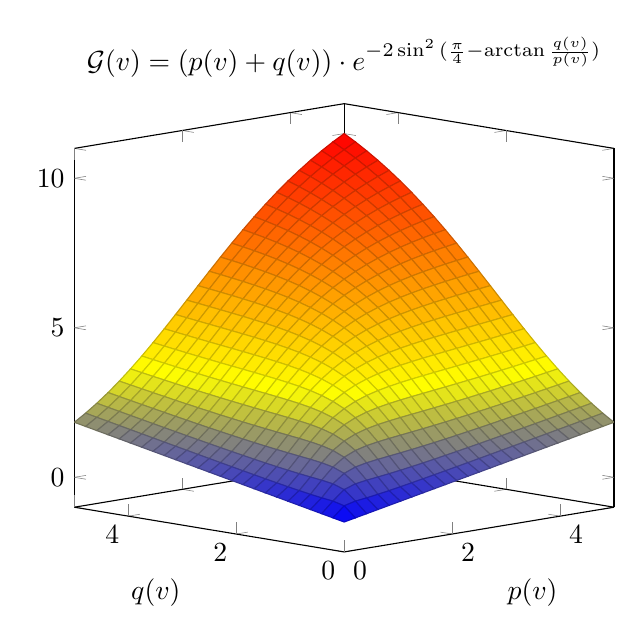
\begin{tikzpicture}[
    declare function={tf(\x)=(pi/4-rad(atan(\x)));},
    declare function={func(\x,\y)=sin(tf(\y/\x)*180/pi);}
]
\begin{axis}[
    view={315}{10},
    title={$
\mathcal{G}(v) = (p(v) + q(v)) \cdot e^{-2\sin^2{(\frac{\pi}{4} -
\arctan\frac{q(v)}{p(v)})}}$},
    xlabel=$p(v)$,
    ylabel=$q(v)$,
]

\addplot3 [
        surf,
        domain=0:5,
        domain y=0:5,
    ] {(x+y)*exp((-2)*(func(x,y))^2)};
\end{axis}
\end{tikzpicture}

	\caption{出入度计算函数曲线 \label{fig-surf}}
\end{figure}
\item 对$G(x,y)$计算Wilbur函数作为出入度最终结果$\beta$。
\end{enumerate}

\section*{AR的计算}
账户的价值AR定义为资产中值指标乘以出入度最终结果,即$\alpha\beta$。

\end{document}
